%
%


\chapter[An introduction to the department's Athena Swan work]{An introduction to the department's\\Athena Swan work}\label{chap:intro}

\vspace*{-1cm}

\instr{In Section 1, applicants should evidence how they meet Criterion A:
\begin{itemize}
\item Structures and processes underpin and recognise gender equality work and, where relevant, wider equality work 
\end{itemize}
Recommended word count: 2000 words
}


\section{Letter of Endorsement from the Head of School}

\instr{
Insert (with appropriate letterhead) a signed letter of endorsement from the head of the department. The letter should comment on:
\begin{itemize}
    \item the link between the Athena Swan Ireland principles and the department's strategy; \item leadership of the head of department in advancing equality, including any involvement in the self-assessment or specific actions; 
    \item evidence of how the department's equality work is led and supported by the department's senior management;
    \item key priorities, achievements and challenges relating to gender equality as discerned from the self-assessment; 
    \item where relevant, key priorities, achievements and challenges relating to additional equality grounds, as discerned from the self-assessment; 
    \item priority actions to address the issues and opportunities identified.
\end{itemize}

}


\begin{mdframed}[backgroundcolor=white,                
                linecolor=black,
                innerleftmargin=1.5cm,
                innerrightmargin=1.5cm,
                innertopmargin=1cm,
                innerbottommargin=1cm,
                usetwoside=false,
                splitbottomskip=2cm,
                splittopskip=2cm,
                everyline=true                
                ]


\sffamily 
\footnotesize

\includegraphics[width=4cm,right]{img/ucclogo.png}\\[.1in]
\begin{tabular}{ll}
\begin{minipage}{8cm}
%TC:ignore
Dr Sara Fink\\
Head of Athena SWAN Ireland\\
Advance HE\\
First Floor, Napier House\\
High Holborn\\
London WC1V 6 AZ\\
United Kingdom\\
%TC:endignore
\end{minipage}
&
\begin{minipage}{4cm}
\tiny  
%TC:ignore
Professor Utz Roedig\\
School of Computer Science and\\Information Technology\\
University College Cork\\
Western Gateway Building\\
Western Road, Cork, Ireland\\
u.roedig@ucc.ie\\
+353 21 420 5900\\
%TC:endignore
\end{minipage}\\
\end{tabular}


30 November, 2022\\[.1in]
Subject: \textbf{Endorsement of Athena SWAN Bronze Award Application}\\[.1in]

Dear Dr Fink,\\

As Head of School of Computer Science and Information Technology (CSIT), I wish to commit my full support to the Athena Swan (AS) Ireland Principles and pledge to imbed these principles into the culture, policies, and practices of the school. In addition to forming an Equality, Diversity, and Inclusivity (EDI) Implementation Committee (EDIIC), each School standing committee will have an Athena Swan Champion; this process will align with the allocation of all school administrative duties.

CSIT is one of the largest schools in the College of Science, Engineering and Food Science (SEFS).  It is a multifaceted ecosystem, composed of academics (33, 9\% female), professional, managerial and support staff (25, 48\% female), research staff (23, 17\% female), postgraduate research (45, 13\% female), postgraduate taught (129, 46\% female) and undergraduate (390, 24\% female) students. 

Traditionally, Computer Science is a male dominated discipline; our flagship undergraduate programme is 14\% female.  Recognising this, we previously formed partnerships with Psychology and Digital Humanities and developed two interdisciplinary undergraduate degrees.  These have been strategically important initiatives which have increased our female undergraduate numbers (24\%). Two female academic staff members have been appointed to teach on, support and develop the gender balance of these programmes. 

We started our AS self-assessment in Spring 2021.  As Head of School, I appointed Professor John Morrison as Chair of the Self-Assessment Team (SAT). Appointing a senior experienced leader as Chair of the SAT demonstrates my commitment supporting the adoption of the AS Principles in the school.  The SAT was composed of 29 school members, 41\% female.  

The SAT has identified five priority areas that will be addressed over the next four years. 

\begin{enumerate}

\item Firstly, we need to develop governance structures, policies and procedures to ensure that the Athena Swan Ireland Principles are embedded in the school.  I will address this priority through the establishment of an EDI Implementation Committee, appointing a Chair from senior staff.  The committee will have the authority to oversee and implement the action plan. 

\item Currently, there is a dearth of female academic (9\%) and research (17\%) staff particularly at higher grades.  Increasing the ratio of female applicants for staff posts in these cohorts is expected to improve the staff gender balance.  I will prioritise the development of guidelines to improve the school's gender imagery and advertising, and actively target females encouraging them to apply for academic and research positions whilst providing focused support for female staff in the school. 

\item Our aim to increase the number of female students registered in undergraduate and postgraduate programmes will continue through ongoing partnerships with our colleagues in digital humanities and psychology. By understanding our current student's motivation to study Computer Science allows us to develop strategies to improve gender balance in our core CS programmes.  We plan to provide a richer experience for our current female students through internships and scholarship, thus providing female role models for future students. 

\item In 2023, I will restart the Performance Development and Review Process (PDRS) to improve support for staff development and career progression.  Mentors will be appointed to female staff and training, and funding workshops will be arranged to enhance their change of promotion.  

\item I am committed to promoting a culture of inclusivity and belonging in the school, and will create a policy defining how the school will implement statutory family leave. I will ensure that students from diverse backgrounds have opportunities to study with us.  We will keep in touch with colleagues from other schools, for example through the \ac{TLCF}, to ensure that we are in line with the EDI agenda both nationally and internationally.

\end{enumerate}

To ensure that our actions are having a positive impact and desired effect on the EDI culture, we will conduct a review towards the end of 2026 to evaluate progress and staff and student satisfaction and experience. 

The information presented in the application is an honest, accurate and true representation of the school. 



Yours sincerely,


\includegraphics[width=1in]{img/signature-roedig.png}

Utz Roedig\\
Professor of Computer Science\\
Head of School of Computer Science and Information Technology

\end{mdframed}



%TC:ignore
\subsubsection{Confirmation}
\textcolor{titlebgdark}{
The information presented in the application (including qualitative and quantitative data) is an honest, accurate and true representation of the department. {\hfill \LARGE \XBox }
}
%TC:endignore

% \begin{labelboxcode}{hello}{Hello world}
% Test 1
% \end{labelboxcode}

\clearpage 
\section{Governance and recognition of equality, diversity and inclusion work}

\subsection{Provide a description of the department's structures to advance equality. This should include:}
\instr{
\begin{itemize}
\item	information on where the department is in the Athena Swan process; 
\item	an organigram of the department's key management and/or committee structures, with headcount by gender, that includes the formal reporting structures in place to carry out and support Athena Swan activity and, if applicable, wider EDI work;
\item	information on the relationship of department structures with departmental Athena Swan structures and, if applicable, EDI structures, including mechanisms for sharing the findings of self-assessment as well as good practice;
\item	information on support provided by the department for the application;  
\item	information on formal processes in place to resource, distribute, recognise and reward Athena Swan and, where applicable, EDI work, referencing department-level policies where appropriate;
\item	resource provision for the action plan and associated activities to ensure effective implementation;
\item	any other relevant structure and organisation information, such as the department's relationship with community partners;
\item	confirmation that staff and students are recorded as the gender with which they identity in this submission.
\end{itemize}
}


\subsubsection{Information on where the department is in the Athena Swan process}

In response to a call for expressions of interest, the school of \ac{CSIT} appointed an \ac{AS} Champion in 2019 in recognition of the importance of the \ac{EDI} agenda at university level, to increase awareness and to set the groundwork to prepare for an AS Bronze application.  Between 2019 and 2022, the Champion represented the school at the College of \ac{SEFS}, and provided regular updates at school meetings. 

A \ac{SAT} was set up in Spring 2021 and all school members were invited to join; the final composition ensured gender representation and role equality among staff and postgraduate students (see Table~\ref{tab:initialexpandedsat}, Page~\pageref{tab:initialexpandedsat}). 

This application reports on three years of data, namely from 2017-2020. 
Data cited in this application have been gathered from a staff survey conducted by the university's \ac{EDI} unit in June-July 2021, and three focus group sessions in May-June 2022. Data maintained as part of local CSIT records are also cited to supplement centralised records. 



\subsubsection{An organigram of the department's key management and/or committee structures, with headcount by gender, that includes the formal reporting structures in place to carry out and support Athena Swan activity and, if applicable, wider EDI work}


Table~\ref{tab:keyroles} summarises leadership roles
within the school, reflecting a dearth of women in senior academic and research grades. 
The term ``Research Director'' in Table~\ref{tab:keyroles} refers to senior
director-level roles in one of the multi-institutional national research centres funded by \ac{SFI} that the school is involved in (Table~\ref{tab:researchcentres}), and two Centres for Research Training (CRT) for training PhD students, also funded by SFI (Table~\ref{tab:crts}). 



\begin{tabbox}{!th}

\caption{Key roles within CSIT by gender}
\label{tab:keyroles}
\footnotesize 

\sisetup{
    group-digits=all,
    group-minimum-digits=4,
    table-format=2.1,
    mode=text,
    reset-text-series = false, 
    text-series-to-math = true,
    reset-text-family=false, 
    text-family-to-math=true
}
\begin{tabular}{p{4cm}
                S[table-format=2.1]
                !{\quad}
                S[table-format=2.1] 
                p{3cm} 
                p{4cm} 
                S[table-format=2.1]
                !{\quad}
                S[table-format=2.0] 
                }
\toprule 
\multicolumn{3}{c}{\textmd{School Leadership}} %JPM Changed Academic to School
&&
\multicolumn{3}{c}{\textmd{Research Leadership}}\\ 
\cmidrule{1-3}\cmidrule{5-7}
& {F} & {M} & & & {F} & {M} \\ 
\midrule 
Head  of School  & 0 & 1 && Research Directors\interdis & 0 & 4\\ %JPM Changed Directors to Research Directors
\cdashline{1-3}\cdashline{5-7}
PMS Managers & 1 & 1& & Principal Investigators & 0& 10\\
\cdashline{1-3}\cdashline{5-7}
%AOD, GP, GR, IP, AZ, MvD, KJS, DM
Programme Directors & 2 & 6 & & SFI Funded Investigators\interdis\interdis & 1& 8\\
\cdashline{1-3}
Committee Chairs& 0 & 8 &&&&\\
\bottomrule 
\end{tabular}
\begingroup
\sffamily 
\singlespacing 
\interdis{} Director refers to Directors or Co-Directors of SFI Research Centres.\\
\interdis\interdis{} SFI Funded Investigator (FI) is a role within an SFI Research Centre, such as Connect and Lero; an FI leads one or more research projects within such a centre, and must be approved by SFI.
\endgroup 

\end{tabbox}

\begin{figbox}{!t}
    \caption{Overall school management and committee structures / programme directors}
    \label{fig:schoolstructure}    
    \centering 
    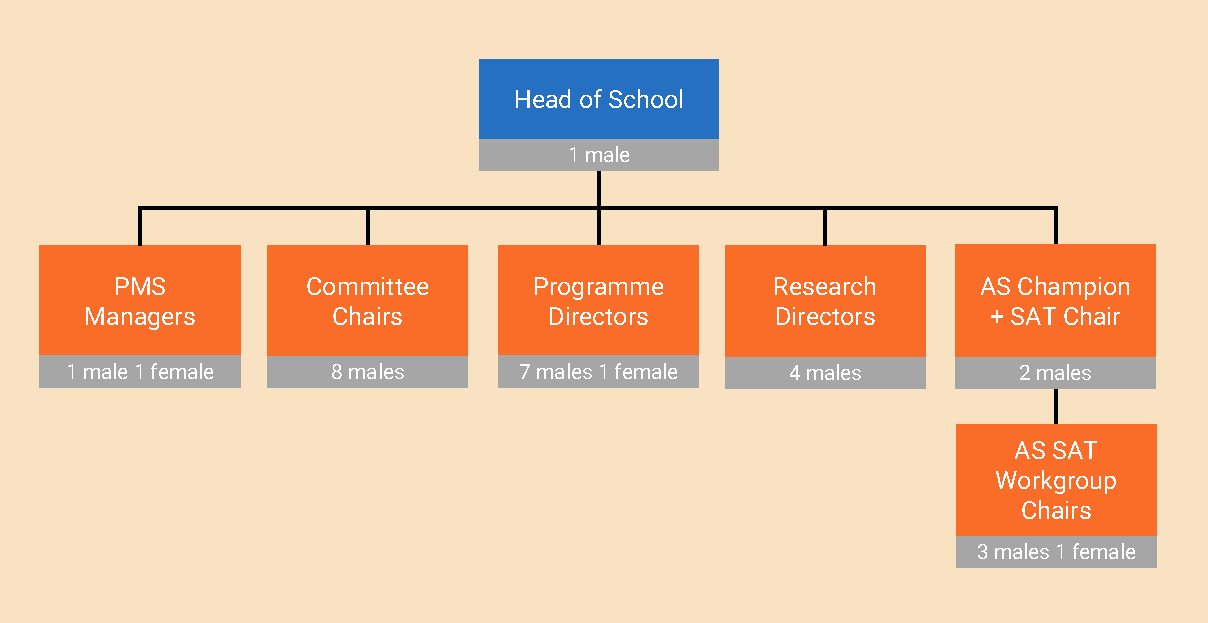
\includegraphics[trim={5mm 5mm 5mm 5mm},clip,width=12cm]{fig/schoolmanagamentdec21.pdf}
\end{figbox}

Figure~\ref{fig:schoolstructure} shows the gender distribution in school leadership roles. Most  staff have administrative responsibilities and serve in school committees.  Key academic administrative responsibilities in the school are clearly gender imbalanced. The greatest gender imbalance is in academic staff, particularly at senior level (Figure~\ref{fig:schoolstaff}).



\begin{figbox}{!ht}
    \caption{School staff at CSIT per Autumn 2022}
    \label{fig:schoolstaff}
    \centering    
    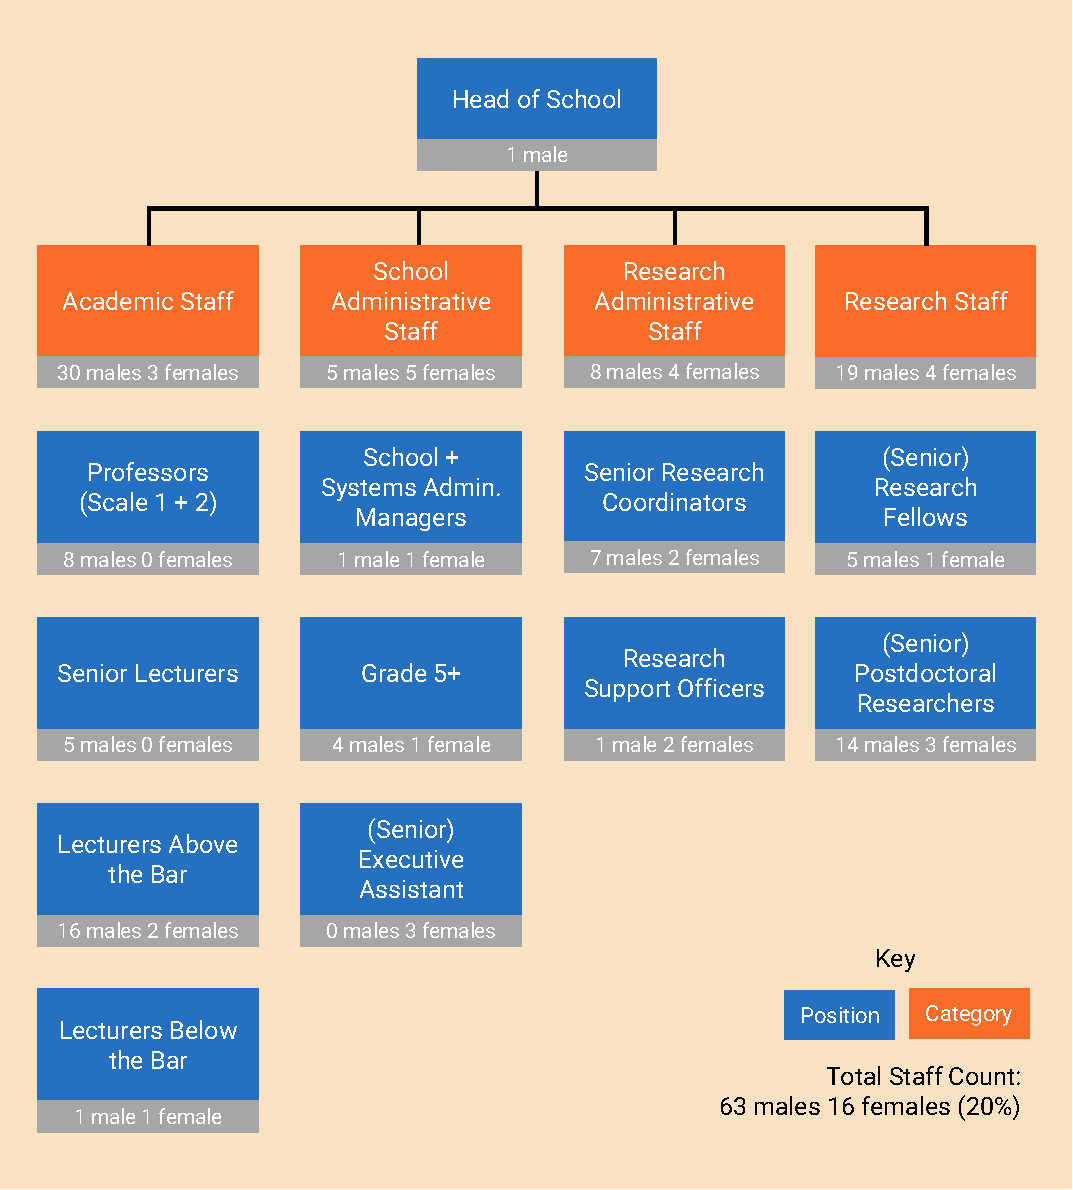
\includegraphics[trim={5mm 5mm 5mm 5mm},clip,width=12cm]{fig/neworganigramDec21.pdf}\\
    {\sffamily\footnotesize \RaggedRight Note: numbers per Autumn 2022; some may differ in other figures and tables.}
\end{figbox}






The school has eight committees to support school activities. 
Table~\ref{tab:gender:committees} shows 
the gender distribution of committee members. 



\begin{tabbox}[11cm]{!th}
\caption{Gender representation in School committees}
\label{tab:gender:committees}
\sisetup{
    group-digits=all,
    group-minimum-digits=4,
    group-separator = {,},
    table-format=4.1,
    mode=text,
    reset-text-series = false, 
    text-series-to-math = true,
    reset-text-family = false, 
    text-family-to-math = true
}
\footnotesize   
\begin{tabular}{p{6cm} 
                !{\quad}
                S[table-format=2.0]
                !{\quad}
                S[table-format=2.0]
                !{\quad}
                S[table-format=2.0\%]
                !{\quad}
                S[table-format=2.0]
                }

\toprule 
Role & {Male} & {Female} & {Female \%} & {Total}\\
\midrule 
Committee Chairs & 8 & 0 & 0\% & 8\\
\hdashline
Committee Members & 16 & 7 & 30\% & 23 \\
\hdashline
All Committee (Chairs and Members) & 24 & 7 & 23\% &31\\
\bottomrule 
\end{tabular}


\end{tabbox}




\subsubsection{Information on the relationship of department structures with departmental Athena Swan structures and, if applicable, EDI structures, including mechanisms for sharing the findings of self-assessment as well as good practice}

The SAT engaged intensively with the university's EDI unit and other schools within the university seeking \ac{AS} accreditation. It also consulted with colleagues in cognate schools from other universities that had already successfully engaged with the AS process. The SAT Chair regularly reported progress through a standing item on the school's monthly meeting agenda.



\subsubsection{Information on support provided by the department for the application}
The school provided full administrative support to the SAT in organising
meetings and taking minutes. The School Manager coordinated the
collection of local data with with the Research Centre administrators
and  compiled this data into a suitable format for the SAT to review.
The \ac{HOS} actively promoted the SAT activities at all school meetings,
encouraging staff to take part in discussions and giving adequate
time for everyone to comment on the process and findings.
In addition, the university provided extensive support to the school during the production of this application. The EDI unit supported in the production, administration and collation of results of the staff survey. In addition, Academic Support Services and HR provided data. Although not required for this application, the university also makes funds available for practical support for AS applications.   


\subsubsection{Information on formal processes in place to resource, distribute, recognise and reward Athena Swan and, where applicable, EDI work, referencing department-level policies where appropriate}

The school recently embarked on its AS journey, so apart from the SAT activities, there are currently no formal processes in place to  resource, distribute, or reward AS work.
At the school level, AS activities are recognised by the \ac{HOS} in assigning administrative workload. On appointment, the Chair was relieved of other administrative obligations to concentrate on coordinating the school's AS activities. 


\subsubsection{Resource provision for the action plan and associated activities to ensure effective implementation}

The school has availed of resources provided by the university's EDI unit for the application, including regular feedback and advice from the university's \ac{AS} Project Officer. It will continue to avail of all centrally available resources to support the implementation of CSIT's Action Plan. The \ac{EDIIC} will report any resource deficits to the \ac{HOS} and to the College's AS Steering Committee.
Appropriate changes to the school structures will seek to support the implementation of the action plan (Actions~\ref{action:intro:edi} and \ref{action:intro:agenda}, Page \pageref{action:intro:edi}),  improving the EDI culture.


\subsubsection{Any other relevant structure and organisation information, such as the department’s relationship with community partners}

Since the school embarked on its AS journey, it has been an active member of the university EDI activities and will benefit from, and contribute to, developing best practice.


\subsubsection{Confirmation that staff and students are recorded as the gender with which they identity in this submission}

All requests by staff or students to record their gender preference have been acceded to with confirmation by all data holders to record the appropriate gender.  

\clearpage 
\section{The Self-Assessment Process}


\subsection{Provide information on the preparation and delivery of this application by the department. This should include:}
\instr{
\begin{itemize}
\item  a description of the self-assessment team\index{self-assessment team}, including comment on the roles and responsibilities of individuals, and how these were assigned. The gender of SAT members, their professional/student role in the department, and their specific role in the SAT should be noted in a table; 
\item	information on how the chair was appointed and on what supports or resources the institution and/or department has given the chair to lead the self-assessment process; 
\item	comment on whether the self-assessment team is representative of the department, including if there is adequate representation of senior staff. 
\end{itemize}
}


\subsubsection{A description of the self-assessment team, including comment on the roles and responsibilities of individuals, and how these were assigned. The gender of SAT members, their professional/student role in the department, and their specific role in the SAT should be noted in a table}

The initial SAT  was appointed in March 2021 after an open invitation by the \ac{HOS} to all school members.
The initial 10 %11 
members were a self-selecting group at various stages in their professional careers and included representation from both Professional Management and Support Staff (PMSS) and Academic staff (see Tables~\ref{tab:initialexpandedsat}).

\begin{tabbox}{!b}
\footnotesize 
\caption{Initial and expanded SAT: Gender, leadership, and staff category}
\label{tab:initialexpandedsat}


\sisetup{
    group-digits=all,
    group-minimum-digits=4,
    group-separator = {,},
    mode=text,
    reset-text-series = false, 
    text-series-to-math = true,
    reset-text-family = false, 
    text-family-to-math = true
}   
\begin{tabular}{p{7cm}
                S[table-format=1.0]
                !{\qquad}
                S[table-format=1.0]
                !{\qquad}
                S[table-format=3.0\%]
                p{0.6cm}
                S[table-format=2.0]
                !{\qquad}
                S[table-format=2.0]
                !{\qquad}
                S[table-format=2.0\%]
                p{0.3cm}
                S[table-format=3.0\%]}
\toprule 

  & \multicolumn{3}{c}{\makecell{Initial SAT\\April 2021}} && \multicolumn{3}{c}{\makecell{Expanded SAT\\December 2021}} && {\makecell{\% by staff\\ category}}\\
  \cmidrule{2-4}\cmidrule{6-8}
  & {M} & {F} & {\%F} && {M} & {F} & {\%F} & \\
  \midrule 
 
Chair 										    & 1 & 0 & 0\% && 1 & 0 & 0\% && {n/a} \\
\hdashline
Workgroup Chairs & 0 & 0 & 0\% && 3 & 1 & 25\% && {n/a}\\
\midrule 
Academic									    & 3 & 2 & 40\% && 12 & 3 & 20\% &&52\% \\
\hdashline
Professional Management and Support Staff & 1 & 4 & 80\% && 3 & 6 & 67\% && 31\%\\
\hdashline
Research staff 								    & 0 & 0 & 0\% &&  2 & 3 & 60\% && 17\%\\
\midrule 
Total 										    & 4 & 6 & 60\% && 17 & 12 & 41\% && 100\%\\
  
\bottomrule 
\end{tabular}

\end{tabbox}

\begin{tabbox}{!b}
\caption{Workgroups and distribution of members by gender and staff category}
\label{tab:wgs}
\sisetup{
    group-digits=all,
    group-minimum-digits=4,
    group-separator = {,},
    table-format=4.1,
    mode=text,
    reset-text-series = false, 
    text-series-to-math = true,
    reset-text-family = false, 
    text-family-to-math = true
}
\footnotesize   
\begin{tabular}{p{8cm} 
                !{\quad}
                S[table-format=2.0]
                !{\quad}
                S[table-format=2.0]
                !{\quad}
                S[table-format=2.0]
                !{\quad}
                S[table-format=2.0]
                !{\quad}
                S[table-format=2.0]
                !{\quad}
                S[table-format=2.0]                            
                }

\toprule 
%& {\multicolumn{2}{c}{Gender}} & {Staff category}\\
       
&\multicolumn{2}{c}{\makecell{Gender}} & & \multicolumn{3}{c}{Staff category}\\      
\cmidrule{2-3}\cmidrule{5-7}
Workgroup & {M} & {F} & & {Academic} & {PMSS} & {Research}\\ 
\midrule 
Chair's Workgroup\textsuperscript{1} & 5 & 2 && 6 & 1 & 0\\
\midrule
WG1:  Department and Its Context & 3 & 1 & & 2 & 2 & 0\\
\hdashline
WG2: Academic and Research Careers & 6 & 3 & & 5 & 0 & 4\\
\hdashline
WG3: Professional, Managerial and Support Staff Careers & 3 & 3 & & 2 & 4 & 0\\
\hdashline
WG4: Inclusion and Belonging & 3 & 3 & & 4 & 1 & 1 \\
\hdashline
Administrative support & 0 & 2 & & 0 & 2 & 0\\
\midrule
Total SAT members (29), by gender, and category\textsuperscript{1} & 17 & 12 && 15 & 9 & 5 \\
\bottomrule 
\end{tabular}
{
\\[2mm]
\sffamily
\textsuperscript{1}Workgroup Chairs are double-counted in the Chair's Workgroup.
}

\end{tabbox}

Midway through the application process, a new Athena Swan Charter was published, including a new application form. 
The SAT responded to these changed by reorganising itself into four thematic Workgroups (WGs) to better match the structure of the new application (see Table~\ref{tab:wgs}). WG Chairs were invited to serve by the SAT Chair, based on their experience in leading teams and knowledge of UCC's institutional structures. WG Chairs were also chosen with the intention of achieving gender balance, although limited by the gender imbalance within the school.

In addition to the four workgroups, a Chair's Workgroup was formed, consisting of the four WG Chairs, the SAT Chair, the School Manager, and the Workgroup Liaison.


Subsequently,  more people were invited 
to join the SAT to maximise representation. This expansion was done by (1) open invitation to all staff, 
and (2) by targeting specific individuals to maximise diversity and promote inclusion. 
The SAT members were at various stages in their career, with many of the senior staff having considerable experience in the running of the school and serving on university committees.
Table~\ref{tab:sat} presents details of all 29 SAT members.\\[.1in]


\clearpage 

%TC:ignore

\newcommand{\mugwidth}{2.7cm}

\begin{mdframed}[backgroundcolor=orangebg,
                 rightline=false,
                 leftline=false,
                 topline=false,
                 bottomline=false,
                 innertopmargin=0pt,
                 ]
\footnotesize                 
\begin{longtable}{P{5cm}
                  !{\qquad}
                  P{\mugwidth}
                  !{\qquad}
                  P{5cm}}
               
\vspace*{-24pt}
\crule{12mm}{3mm}\\[-7mm]

\caption{Athena Swan Self Assessment Team}\label{tab:sat}\\
\toprule
    Name and Position & & Role on SAT\\
\midrule
\endfirsthead
%
\endhead
%
\endfoot
\bottomrule 
\endlastfoot



John Morrison (M) Professor & 
\adjustbox{valign=t}{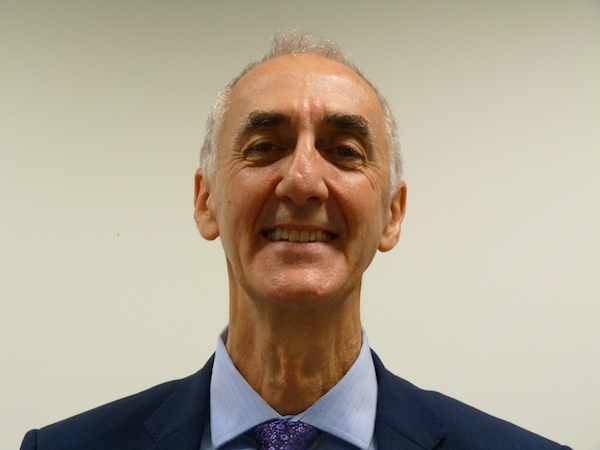
\includegraphics[width=\mugwidth]{img/johnmor.JPG}} & Chair of the CSIT Self-Assessment Team, Member of the Editorial Team \\

\addlinespace
\hdashline

Margaret Hynes (F) Executive Assistant & 
\adjustbox{valign=t}{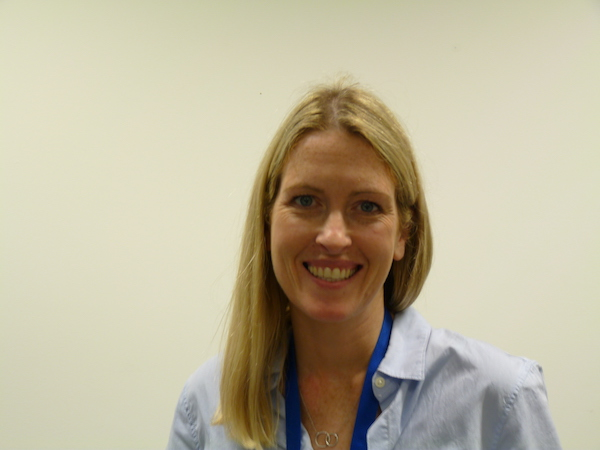
\includegraphics[width=\mugwidth]{img/margaret.JPG}} & SAT Administrative support \\


\addlinespace
\hdashline

Klaas-Jan Stol (M) Lecturer, Funded Investigator at Lero Research Centre, Supervisor at ADVANCE-CRT & 
\adjustbox{valign=t}{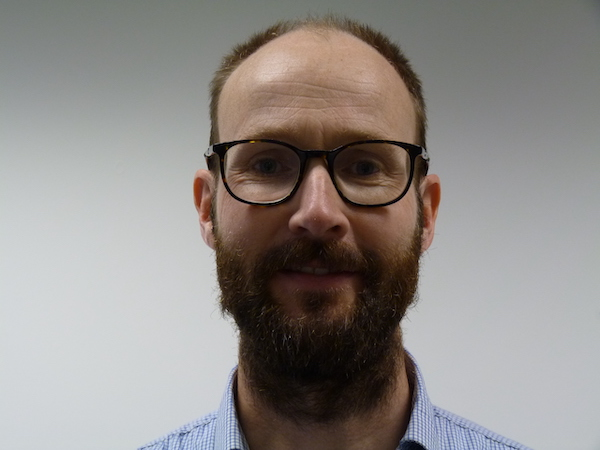
\includegraphics[width=\mugwidth]{img/klaas.JPG}} & Workgroup Liaison; data visualisation, SAT document manager. Member of the Chair's Workgroup, Member of the Editorial Team\\

\addlinespace
\hdashline




Julie Walsh (F) Executive Assistant  & 
\adjustbox{valign=t}{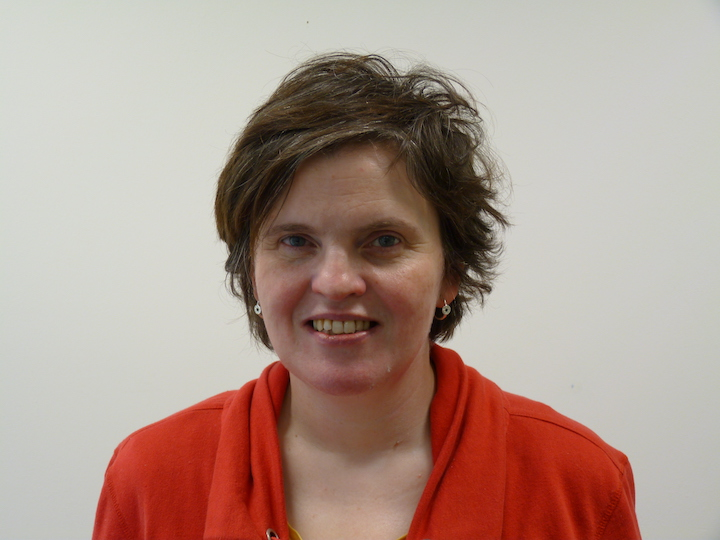
\includegraphics[width=\mugwidth]{img/Julie.JPG}} & SAT Administrative support\\



\addlinespace
\midrule
\multicolumn{3}{c}{Workgroup 1: Department and Its Context }\\
\midrule 

Kieran Herley (M) Lecturer, Chair of the Academic Programmes and Curriculum Development Committee (APCD) & 
\adjustbox{valign=t}{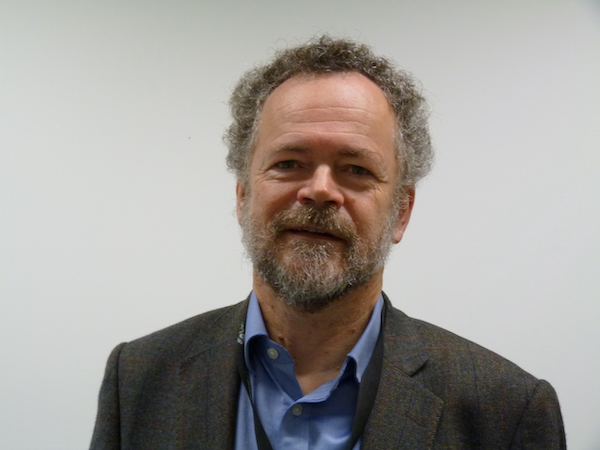
\includegraphics[width=\mugwidth]{img/kieran.JPG}} & Chair of Workgroup 1: Department and Its Context \\

\addlinespace   
\hdashline



Martin Moriarty (M) Systems Administrator &
 \adjustbox{valign=t}{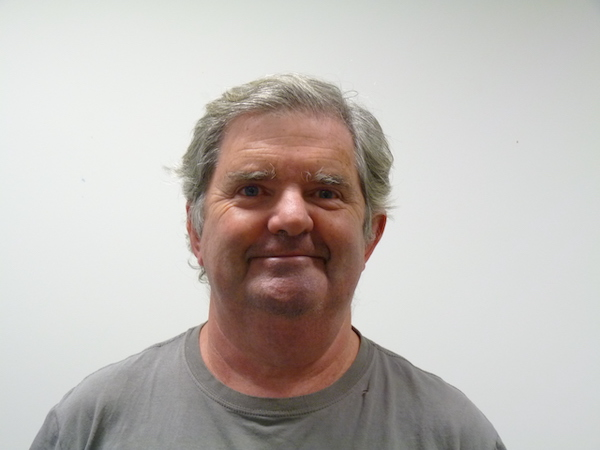
\includegraphics[width=\mugwidth]{img/martin.JPG}} & Member of Workgroup 1: Department and Its Context\\

\addlinespace
\hdashline


John O'Mullane (M) Lecturer &    
\adjustbox{valign=t}{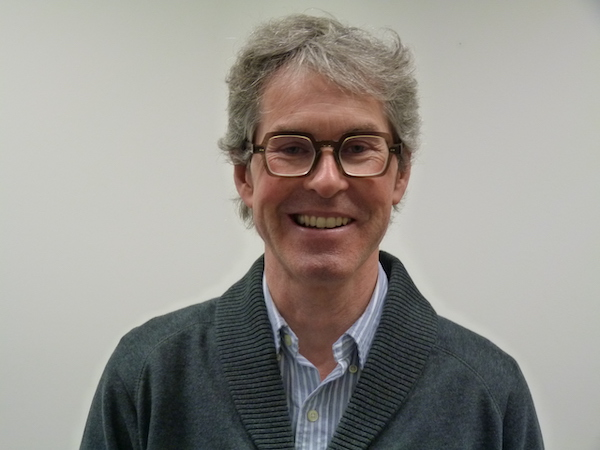
\includegraphics[width=\mugwidth]{img/johnom.JPG}} & Member of Workgroup 1: Department and Its Context \\

\addlinespace 
\hdashline 

Derbhile Timon (F) School Manager &
\adjustbox{valign=t}{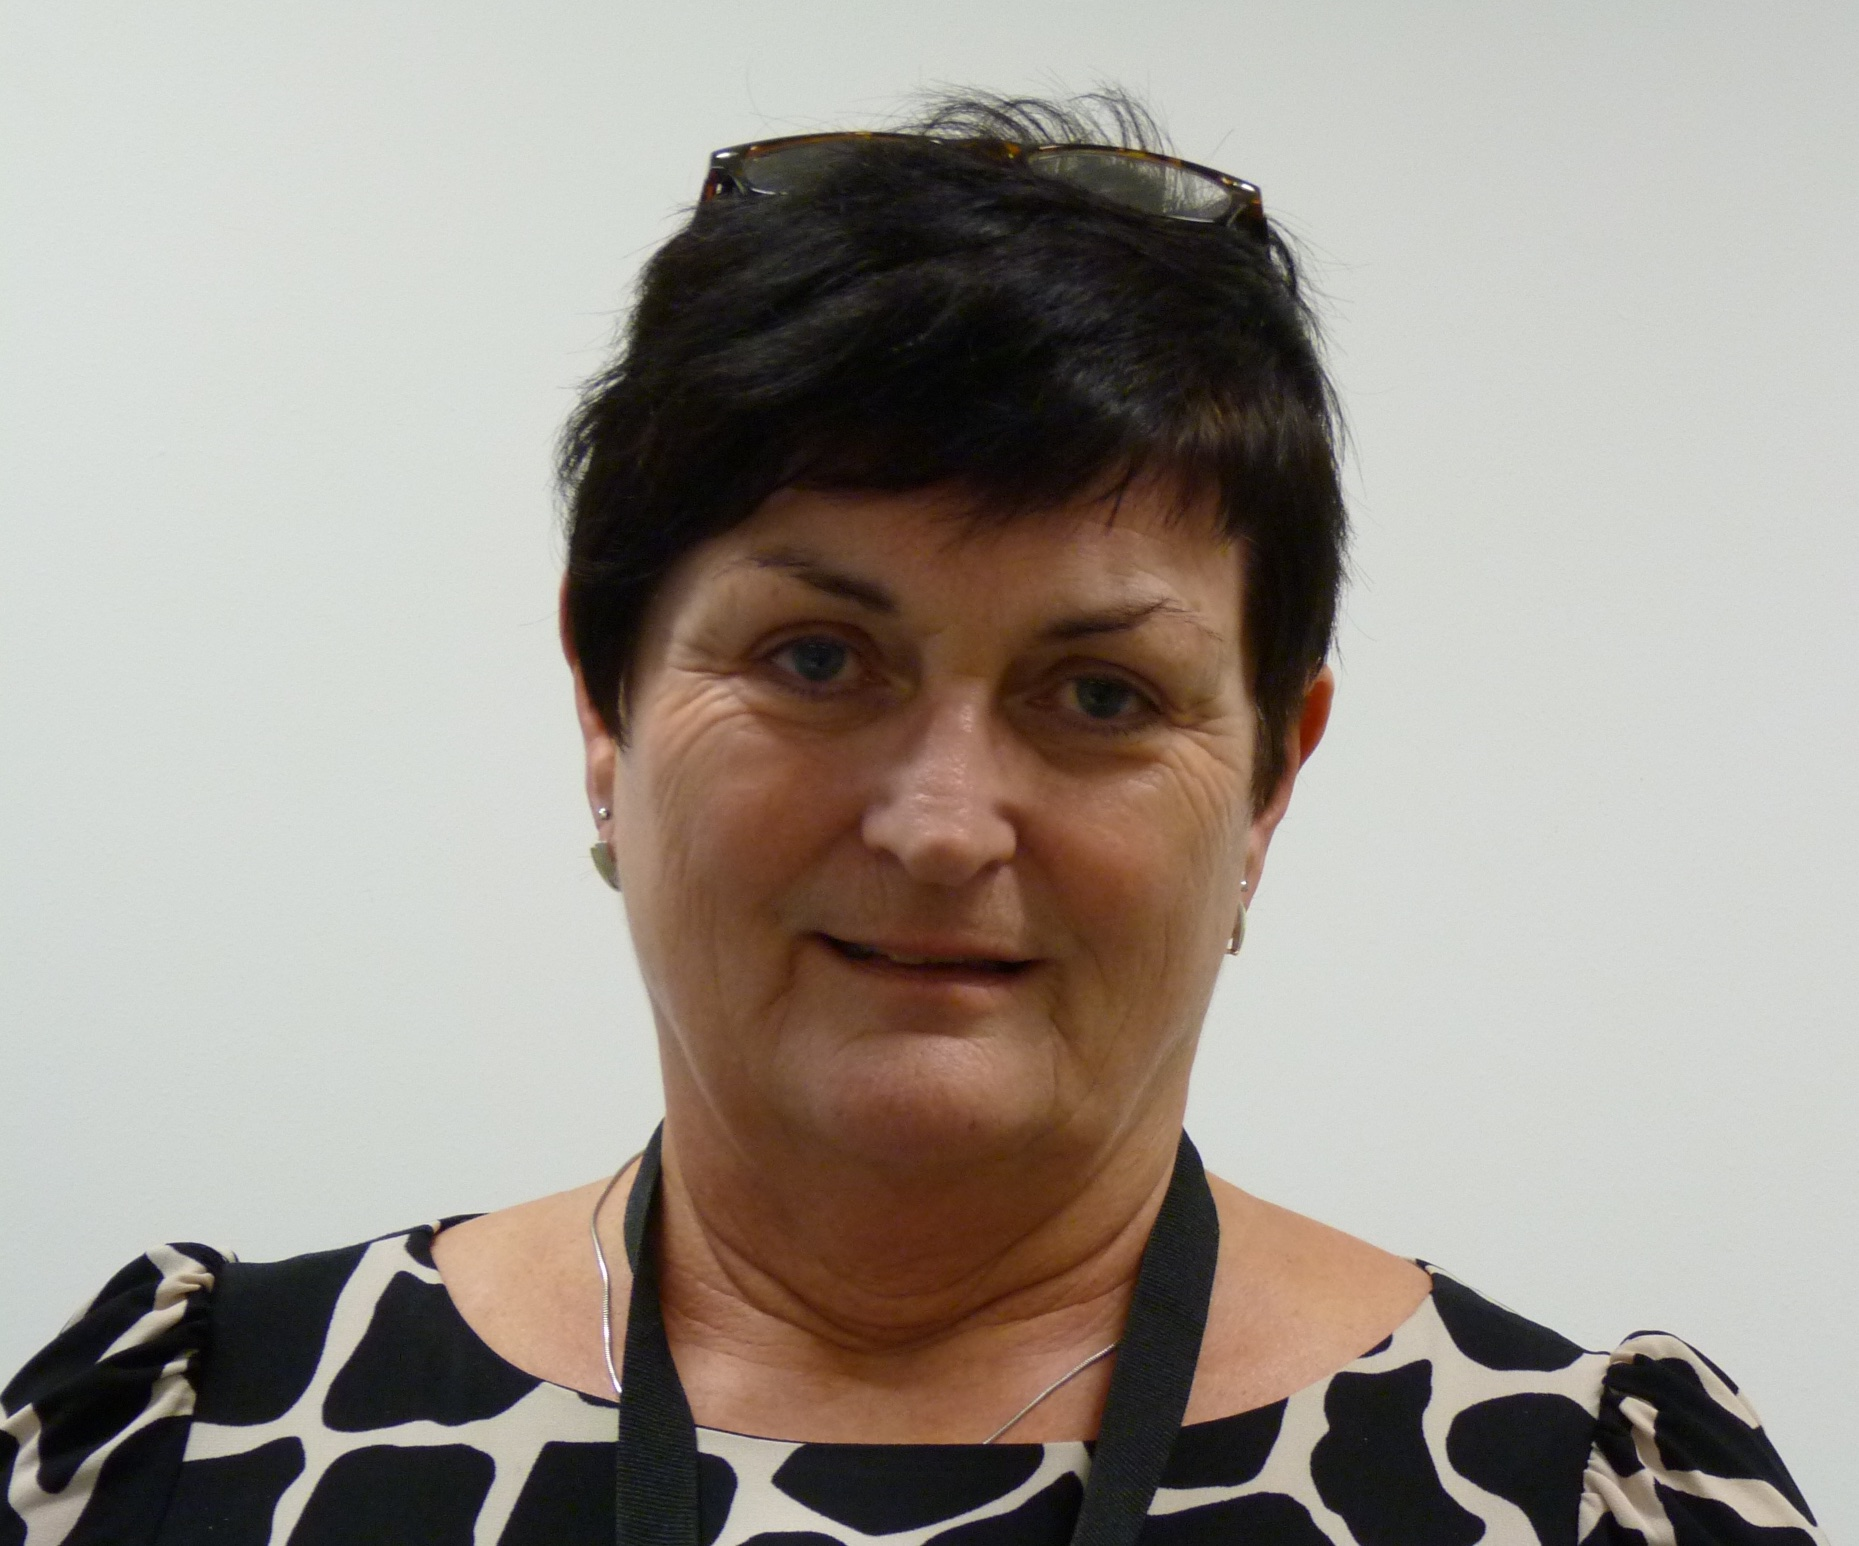
\includegraphics[width=\mugwidth]{img/derbhile.JPG}} & Member of Workgroup 1: Department and Its Context. Member of the Chair's Workgroup, Member of the Editorial Team \\


\addlinespace

\midrule
\multicolumn{3}{c}{Workgroup 2: Academic and Research Careers}\\
\midrule 

Dirk Pesch (M) Professor, Director of ADVANCE-CRT, Co-PI with Connect and Confirm Research Centres; Steering Committee Member of SFI Enable Spoke & \adjustbox{valign=t}{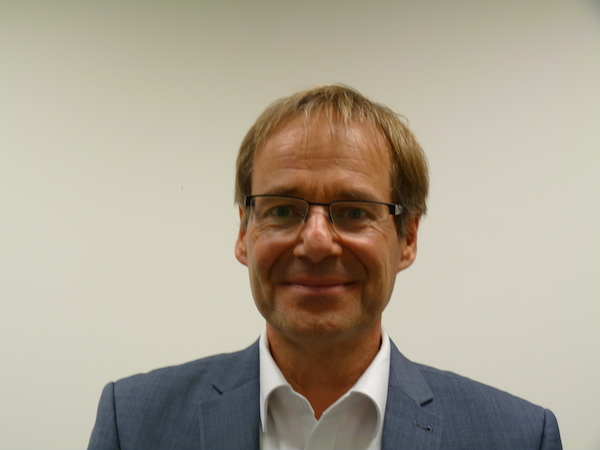
\includegraphics[trim={10mm 0 0 10mm},clip,width=\mugwidth]{img/dirk.JPG}} & Chair of Workgroup 2: Academic and Research Careers. Member of the Chair's Workgroup \\

\addlinespace
\hdashline

Vlad Ionescu (M) PhD Candidate &
\adjustbox{valign=t}{
\includegraphics[width=\mugwidth]{img/vlad.jpg}} & Member of Workgroup 2: Academic and Research Careers\\

\addlinespace
\hdashline

Buvana Ganesh (F) PhD Candidate &
\adjustbox{valign=t}{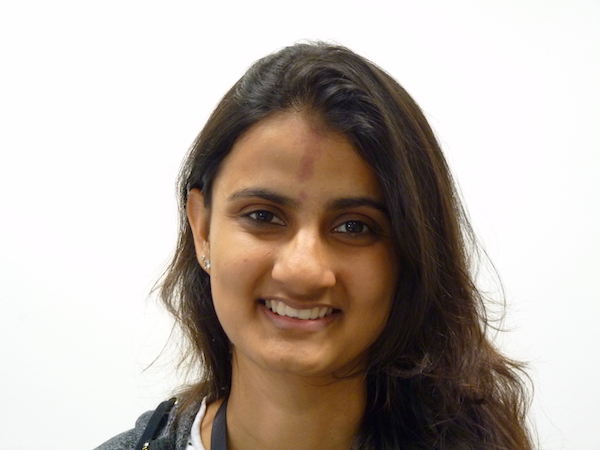
\includegraphics[width=\mugwidth]{img/buvana.JPG}} &Member of Workgroup 2: Academic and Research Careers \\

\addlinespace
\hdashline

Md. Noor-A-Rahim (M) Research Fellow & 
\adjustbox{valign=t}{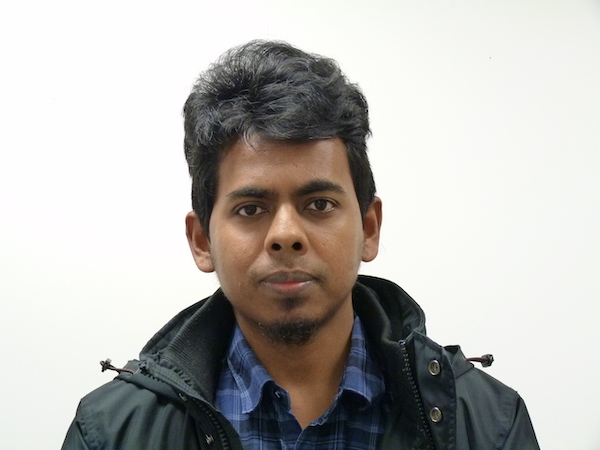
\includegraphics[width=\mugwidth]{img/md.JPG}} & Member of Workgroup 2: Academic and Research Careers \\

\addlinespace
\hdashline

Jason Quinlan (M) Lecturer &
\adjustbox{valign=t}{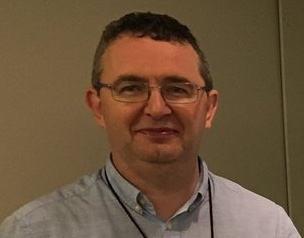
\includegraphics[trim={0 3mm 0 0},clip,width=\mugwidth]{img/jason.JPG}} & Member of Workgroup 2: Academic and Research Careers \\

\addlinespace
\hdashline



Rosane Minghim (F) Lecturer, Supervisor with ADVANCE-CRT & 
\adjustbox{valign=t}{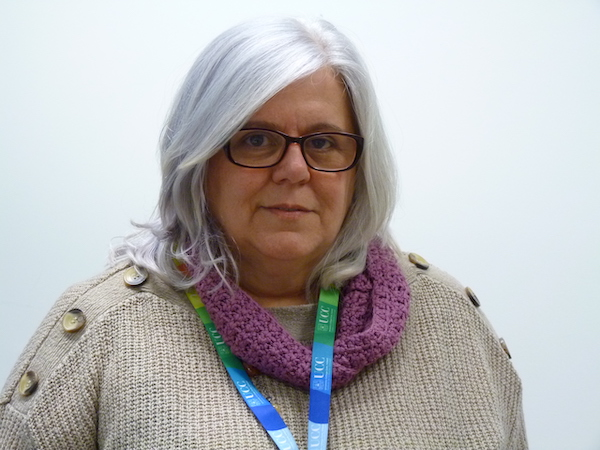
\includegraphics[width=\mugwidth]{img/rosanne.JPG}} & Member of Workgroup 2: Academic and Research Careers\\

\addlinespace
\hdashline


Beg\"{u}m Gen\c{c} (F) Postdoctoral researcher at Insight, now moved to Apple & 
\adjustbox{valign=t}{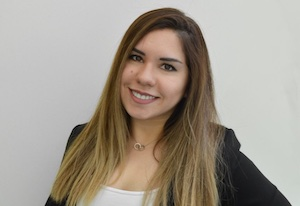
\includegraphics[width=\mugwidth]{img/begum.jpg}} & Member of Workgroup 2: Academic and Research Careers\\

\addlinespace
\hdashline

Barry O'Sullivan (M) Professor, Director of Insight Research Centre, co-PI with Confirm Research Centre &    
\adjustbox{valign=t}{
\includegraphics[trim={0 10mm 0 3mm},clip,width=\mugwidth]{img/barry.JPG}} & Member of Workgroup 2: Academic and Research Careers\\
    
\addlinespace   
\hdashline 

Andrea Visentin (M) Lecturer & 
\adjustbox{valign=t}{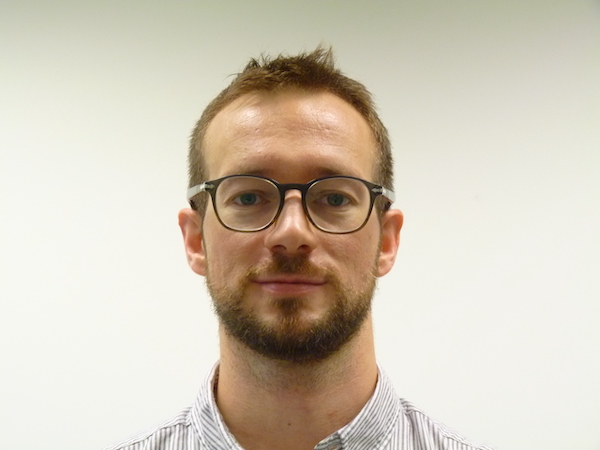
\includegraphics[width=\mugwidth]{img/andrea.JPG}} & Member of Workgroup 2: Academic and Research Careers\\

\addlinespace

\midrule
\multicolumn{3}{c}{Workgroup 3: Professional, Managerial and Support Staff Careers}\\
\midrule 

Aisling O'Driscoll (F) Lecturer, Course Director of BSc Computer Science (BScCS), Funded Investigator at Connect Research Centre, Supervisor at ADVANCE-CRT &
\adjustbox{valign=t}{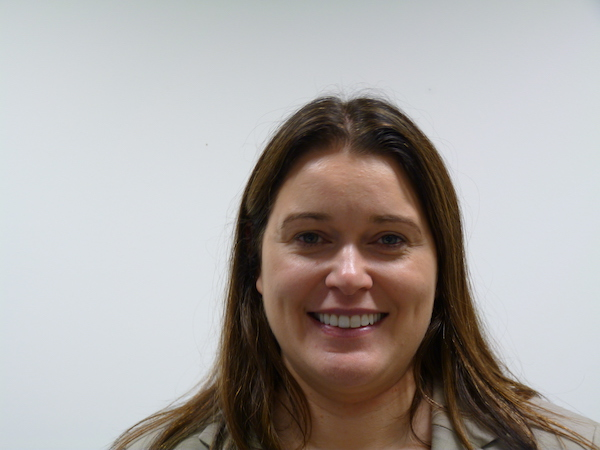
\includegraphics[trim={10mm 0 0 10mm},clip,width=\mugwidth]{img/aisling.JPG}} & Chair Workgroup 3: Professional, Managerial and Support Staff Careers. Member of the Chair's Workgroup\\

\addlinespace
\hdashline

James Duggan (M) Senior Executive Assistant, ADVANCE-CRT &
\adjustbox{valign=t}{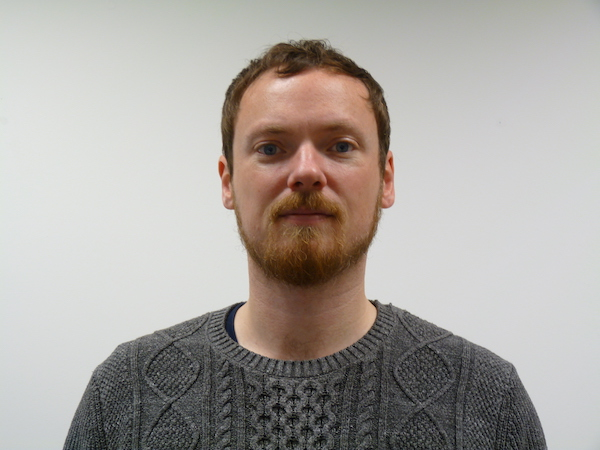
\includegraphics[width=\mugwidth]{img/jamesduggan.JPG}} & Member of Workgroup 3: Professional, Managerial and Support Staff Careers\\

\addlinespace
\hdashline


David O'Byrne (M) Computing Systems Manager & 
\adjustbox{valign=t}{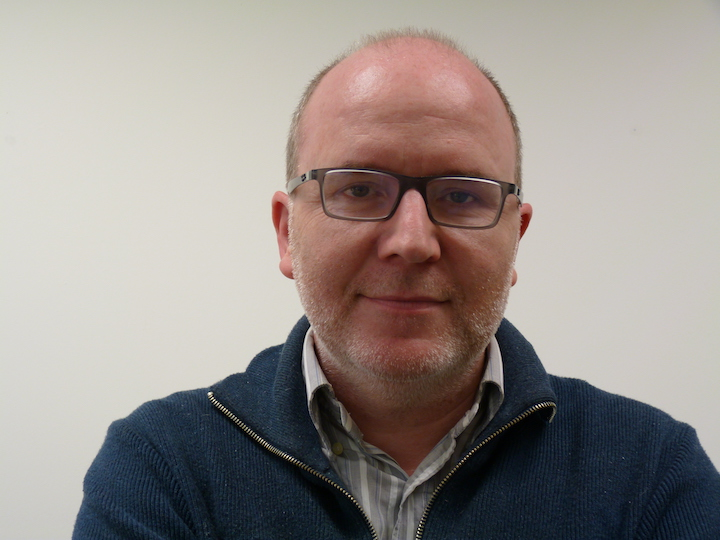
\includegraphics[width=\mugwidth]{img/DavidOB.JPG}} & Member of Workgroup 3: Professional, Managerial and Support Staff Careers \\

\addlinespace    
\hdashline

Adrian O'Riordan (M) Lecturer & 
\adjustbox{valign=t}{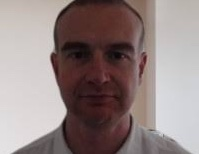
\includegraphics[width=\mugwidth]{img/adrian.jpg}} & Member of Workgroup 3: Professional, Managerial and Support Staff Careers\\
  
\addlinespace
\hdashline

Eleanor O'Riordan (F) Administrator with Insight Research Centre &    
\adjustbox{valign=t}{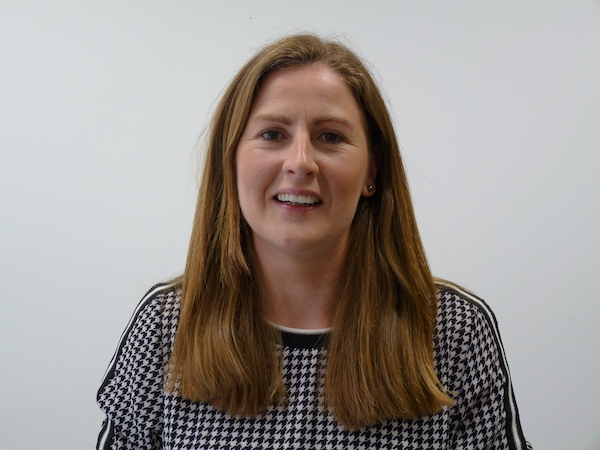
\includegraphics[width=\mugwidth]{img/eleanor.JPG}} & Member of Workgroup 3: Professional, Managerial and Support Staff Careers\\

\addlinespace
\hdashline 


Youngsin O'S\'{e} (F) Senior Executive Assistant  &    
\adjustbox{valign=t}{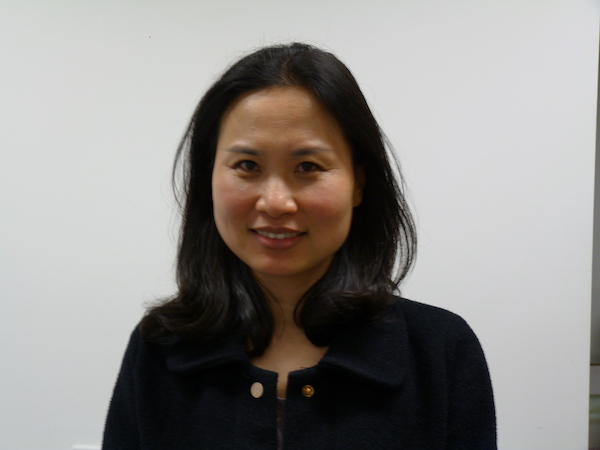
\includegraphics[trim={2mm 2mm 4mm 0},clip,width=\mugwidth]{img/youngsin.JPG}} & Member of Workgroup 3: Professional, Managerial and Support Staff Careers\\

\addlinespace
\pagebreak 
\midrule
\multicolumn{3}{c}{Workgroup 4: Inclusion and Belonging}\\
\midrule 

Paolo Palmieri (M) Lecturer, Funded Investigator at Connect  and Insight Research Centres, Supervisor at ADVANCE-CRT and CRT-AI & 
\adjustbox{valign=t}{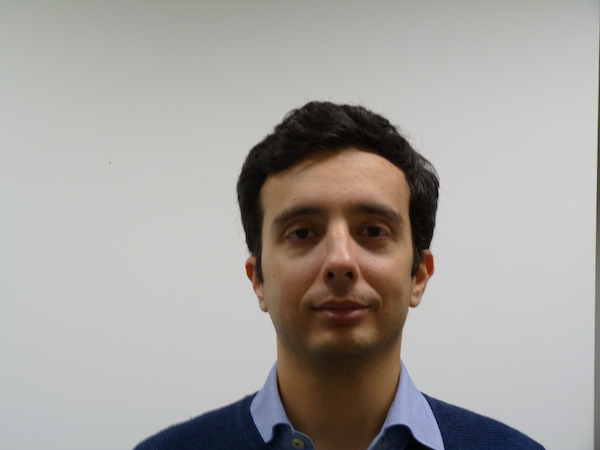
\includegraphics[trim={20mm 0 10mm 16mm},clip,width=\mugwidth]{img/paolo.JPG}} & Chair of Workgroup 4: Inclusion and Belonging. Member of the Chair's Workgroup\\

\addlinespace   
\hdashline 

Andrea Balogh (F) PhD Candidate & %% left low right up
\adjustbox{valign=t}{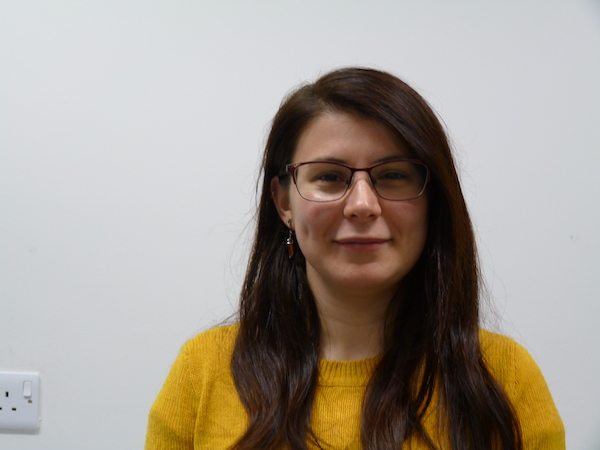
\includegraphics[trim={20mm 10mm 0 10mm},clip,width=\mugwidth]{img/andrea2.JPG}} & Member of Workgroup 4: Inclusion and Belonging\\


\addlinespace
\hdashline


Laura Maye (F) Lecturer, Course Director BA Psychology \& Computing (BAPC), Supervisor with ADVANCE-CRT &
\adjustbox{valign=t}{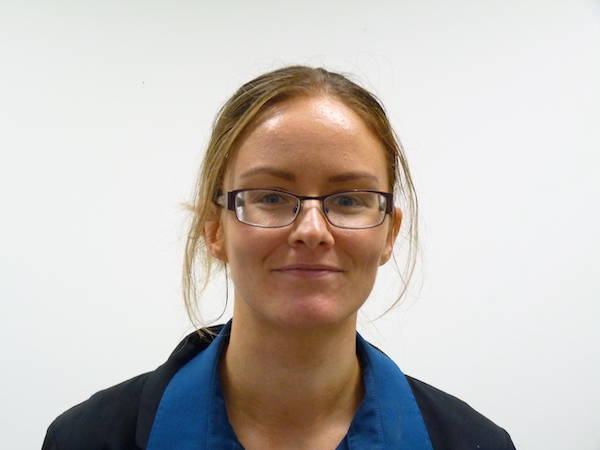
\includegraphics[width=\mugwidth]{img/laura.JPG}} & Member of Workgroup 4: Inclusion and Belonging\\

\addlinespace
\hdashline


Joanne Murphy (F) Administrative Officer &   
\adjustbox{valign=t}{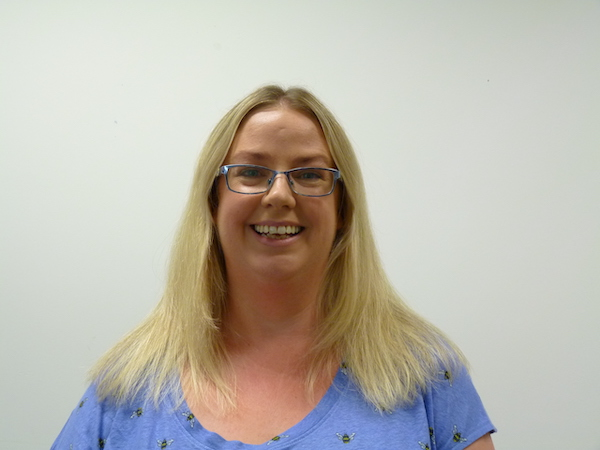
\includegraphics[width=\mugwidth]{img/joanne.JPG}} & Member of Workgroup 4: Inclusion and Belonging\\

\addlinespace
\hdashline

Sabin Tabirca (M) Senior Lecturer, Supervisor at ADVANCE-CRT, Coordinator of the Munster Programming Training (MPT) & 
\adjustbox{valign=t}{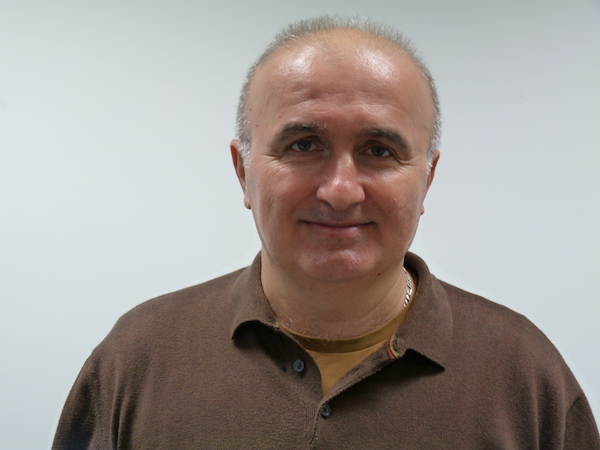
\includegraphics[width=\mugwidth]{img/sabin.JPG}} & Member of Workgroup 4: Inclusion and Belonging\\

\addlinespace
\hdashline
  
Ahmed Zahran (M) Lecturer, Course Director MSc Data Science and Analytics (MScDSA), Funded Investigator Connect Research Centre, Supervisor at ADVANCE-CRT &
\adjustbox{valign=t}{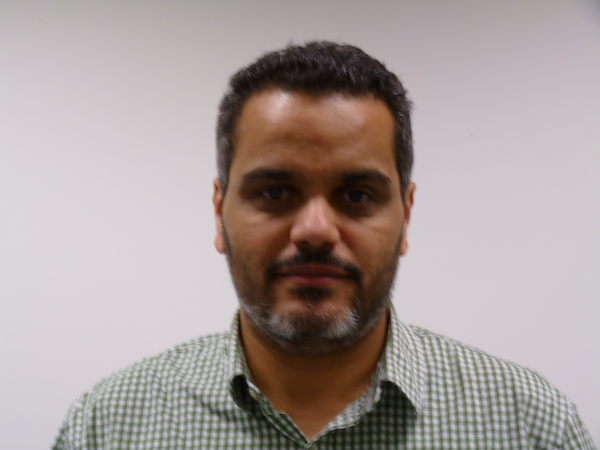
\includegraphics[width=\mugwidth]{img/ahmed.JPG}} & Member of Workgroup 4: Inclusion and Belonging\\

\bottomrule 


\end{longtable}
\end{mdframed}

%TC:endignore


\subsubsection{Information on how the chair was appointed and on what supports or resources the institution and/or department has given the chair to lead the self-assessment process}

Following an open invitation, in March 2021, 
the \ac{HOS} appointed Prof. Morrison to SAT Chair. Prof. Morrison has over 30 years experience of successfully leading large national and international research programmes and was recognised in 2017 by Enterprise Ireland as a Champion of EU Research. 
The Chair was supported by the School Manager and the Workgroup Liaison, who liaised with WG Chairs to analyse and visualise data, and compiled the application document.



\subsubsection{Comment on whether the self-assessment team is representative of the department, including if there is adequate representation of senior staff}

All of the female academic staff members and over 50\% of female PMS staff were members of the SAT. 
In total 41\% of the SAT were female.
Six members (21\%) of the SAT were senior staff, including 3 Professors, 1 Senior Lecturer, 1 Systems Administration Manager, and 1 School Manager. 


\subsection{Provide information on the preparation and delivery of this application by the department. This should include:}
\instr{
\begin{itemize}
\item an overview of the approach taken to evidence-gathering and analysis. Details of consultation response rates, disaggregated by gender, should be provided;
\item	information on plans for evaluating progress, including action plan implementation, over the coming four-year period. This should make reference to how often the SAT will meet, and how SAT succession and turnover will be planned and managed; 
\item	information on how the findings and activity of the self-assessment team are, and will continue to be, communicated to senior management and the wider department.
\end{itemize}
}


\subsubsection{An overview of the approach taken to evidence-gathering and analysis. Details of consultation response rates, disaggregated by gender, should be provided}

The SAT held several orientation meetings in April and May of 2021 to understand the scope of the AS process and to share ideas and experiences. Meetings were also held between UCC's EDI unit and the SAT Chair. 


At the time the SAT was formed, Covid-19 restrictions were in full force. A Microsoft Teams channel was created for the SAT, and all SAT meetings were conducted online.
All staff responded positively to the challenges of working remotely.


The SAT began working with the standard survey provided by the EDI unit; this was augmented to allow for more in-depth feedback.
Questions were added on parental leave, on experiences of new staff and on experiences of staff from under-represented groups. 




\begin{tabbox}{!t}

\caption{Survey response by gender, compared to total School staff count and gender distribution, and response rate by gender}
\label{tab:response:bygender}
\sisetup{
    group-digits=all,
    group-minimum-digits=4,
    group-separator = {,},
    table-format=4.1,
    mode=text,
    reset-text-series = false, 
    text-series-to-math = true,
    reset-text-family = false, 
    text-family-to-math = true
}
\footnotesize   
\begin{tabular}{p{4.5cm} 
                !{\qquad}
                S[table-format=2.0]
                !{\quad}
                S[table-format=2.1\%]
                p{0.5cm}
                S[table-format=2.0\%]                 
                !{\quad}
                S[table-format=2.1\%] 
                !{\qquad}
                S[table-format=2.1\%]                 
                } 

\toprule 
    & \multicolumn{2}{c}{\makecell{Gender representation\\of survey respondents}} 
    &
    & \multicolumn{2}{c}{\makecell{Gender representation\\of all staff School of CSIT}} 
    & {\multirow{2}{2cm}{\makecell{Overall\\Response\\rate}}}\\
    \cmidrule{2-3}\cmidrule{5-6}
Gender & {Count} & {\%} && {Count} & {\%} &  \\ 
\midrule 
Female & 16 & 28.6\% &&  19 & 23.5\% & 84.2\%\\
\hdashline
Male & 37 & 66.1\% && 62 &  76.5\% &59.7\%\\
\hdashline
Prefer not to say & 3 & 5.4\% && {n/a} & {n/a} & {n/a}\\
\midrule 
Total & 56 & 100.0\% && 81 & 100.0\% &69.1\%\\
\bottomrule 
\end{tabular}


\end{tabbox}


% \begin{SCfigure}[10][!ht]
% \hspace{-3pt}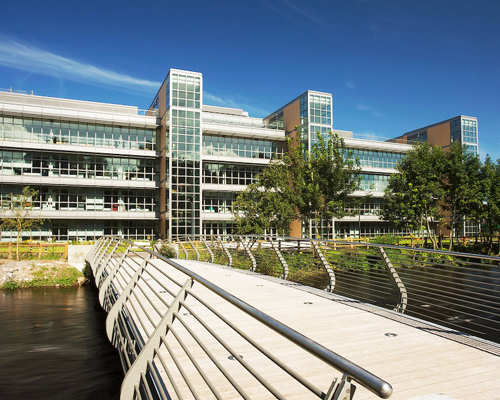
\includegraphics[width=3in]{img/WGB.jpg}
% \caption{Western Gateway Building: home to CSIT}
% \label{fig:wgb}
% \end{SCfigure}




\begin{tabbox}{!th}
\caption{Survey response by role}
\label{tab:response:byrole}
\sisetup{
    group-digits=all,
    group-minimum-digits=4,
    group-separator = {,},
    table-format=4.1,
    mode=text,
    reset-text-series = false, 
    text-series-to-math = true,
    reset-text-family = false, 
    text-family-to-math = true
}
\footnotesize   
\begin{tabular}{p{6.0cm} 
                !{\qquad}
                S[table-format=2.0]
                !{\quad}
                S[table-format=2.1\%]
                p{0.5cm}                
                S[table-format=2.0]
                !{\quad}
                S[table-format=3.2\%]
                p{0.5cm}                
                S[table-format=2.0]
                !{\quad}
                S[table-format=3.1\%]
                }

\toprule 
&\multicolumn{2}{c}{\makecell{Total survey\\ responses}}&&\multicolumn{2}{c}{\makecell{Female survey\\responses}}&&\multicolumn{2}{c}{\makecell{Male survey\\ responses}}\\
\cmidrule{2-3}\cmidrule{5-6}\cmidrule{8-9}
Category & {Count} & {\%} && {Count} & {\%} && {Count} & {\%}\\
\midrule 
Professional, Managerial and Support Staff & 14 & 25.0\% && 8 & 50.00\% && 6 & 16.2\%\\
\hdashline
Research Staff	& 16	 & 28.6\%	& & 7	& 43.75\%	&& 9	& 24.3\%\\
\hdashline
Academic Staff	& 21	& 41.1\%	&& 1 &	6.25\%	&& 20	&54.1\%\\
\hdashline
Teaching Staff	& 2	& 5.4\%	&& 0	& 0.00\%	&& 2	& 5.4\%\\
\midrule
Total & 53\textsuperscript{1} & 100.0\% && 16 & 100.00\% & & 37 & 100.0\%\\
\bottomrule 
\end{tabular}
{\\[.1in]
\sffamily
\textsuperscript{1} Three respondents preferred not to state their gender, which explains the discrepancy with Table~\ref{tab:response:bygender}.
}
\end{tabbox}

There were 56 responses, giving a participation rate of 69\%.  The response rates by gender for academic and \ac{PMS} staff reflect the gender balance in the school. Tables~\ref{tab:response:bygender} and \ref{tab:response:byrole} present the response rates by gender and by role. Those who did not disclose their gender (`prefer not to say') did not identify their role in the school. 

Responses to certain questions were low.
Following an invitation to all staff, 12 colleagues participated in 
three focus group sessions (for academic, PMS, and research staff) that were organised in May-June 2022, covering the following topics:

\begin{enumerate}[noitemsep]
\item Flexible working;
\item Support for colleagues with caring obligations; 
\item Support for career progression and development; 
\item School culture.
\end{enumerate}



Furthermore, four one-on-one interviews were undertaken with School Management.
Institutional data were provided by \ac{HR} and Central Academic Services. The university's EDI unit mediated all data, ensuring proper procedures and policies were applied.  



All WG activity and meeting minutes were stored and shared through the dedicated Microsoft Teams channel. This unrestricted access to data helped to support communications across the entire SAT. 


Each WG met weekly. The Chair's Workgroup met fortnightly, briefed each other on the activities of the previous period, coordinated cross-cutting WG activities, and planned actions for the coming period. 
The entire SAT met monthly and were briefed by the WG Chairs. Feedback from the entire SAT was invited, and was considered by each WG in subsequent meetings. Every effort was made to ensure that the SAT meetings were inclusive and open to diverse opinions.
The SAT meetings were timed to precede the monthly school meeting, where an update on SAT activities was a standing item on the agenda.
Figure~\ref{fig:timeline} shows the SAT activity timeline.

Members of the SAT took part in the online AdvanceHE training seminars and colleagues from schools and universities who were successful in achieving AS accreditation gave generously of their time to talk to the SAT and to share their experiences, including Professor Ita Richardson (University of Limerick), and Professor Lucy Hederman (Trinity College Dublin).







\subsubsection{Information on plans for evaluating progress, including action plan implementation, over the coming four-year period. This should make reference to how often the SAT will meet, and how SAT succession and turnover will be planned and managed}

In 2023,  the school structure will be augmented with the \ac{EDIIC}, thus replacing the AS SAT. It will be chaired by a senior member of staff and having male and female representation from academic, \ac{PMS}, and research staff (Action~\ref{action:intro:edi}). 



\begin{actionblock}{\ksspace{}Establish an EDI Implementation Committee}{intro:edi}
\actintroedi
\hfill{
    \hypersetup{hidelinks}
    \hyperlink{a2}{\gotoactionsymbol{}}
}
\end{actionblock}



Succession planning and turnover of the EDIIC membership will be managed by the \ac{HOS}, biennially using the same mechanisms for all other administrative appointments. Each member of the EDIIC will be also be a member of one of the School Standing  Committees: the \ac{APCD}; the Graduate Studies; Outreach; Research; Teaching and Learning; and the Student Experience. There they will act as an EDI champion, highlighting issues of concern.


\begin{landscape}

\begin{figbox}[20cm]{!ht}

    \caption{Timeline of events}
    \label{fig:timeline}
    % left low right up
    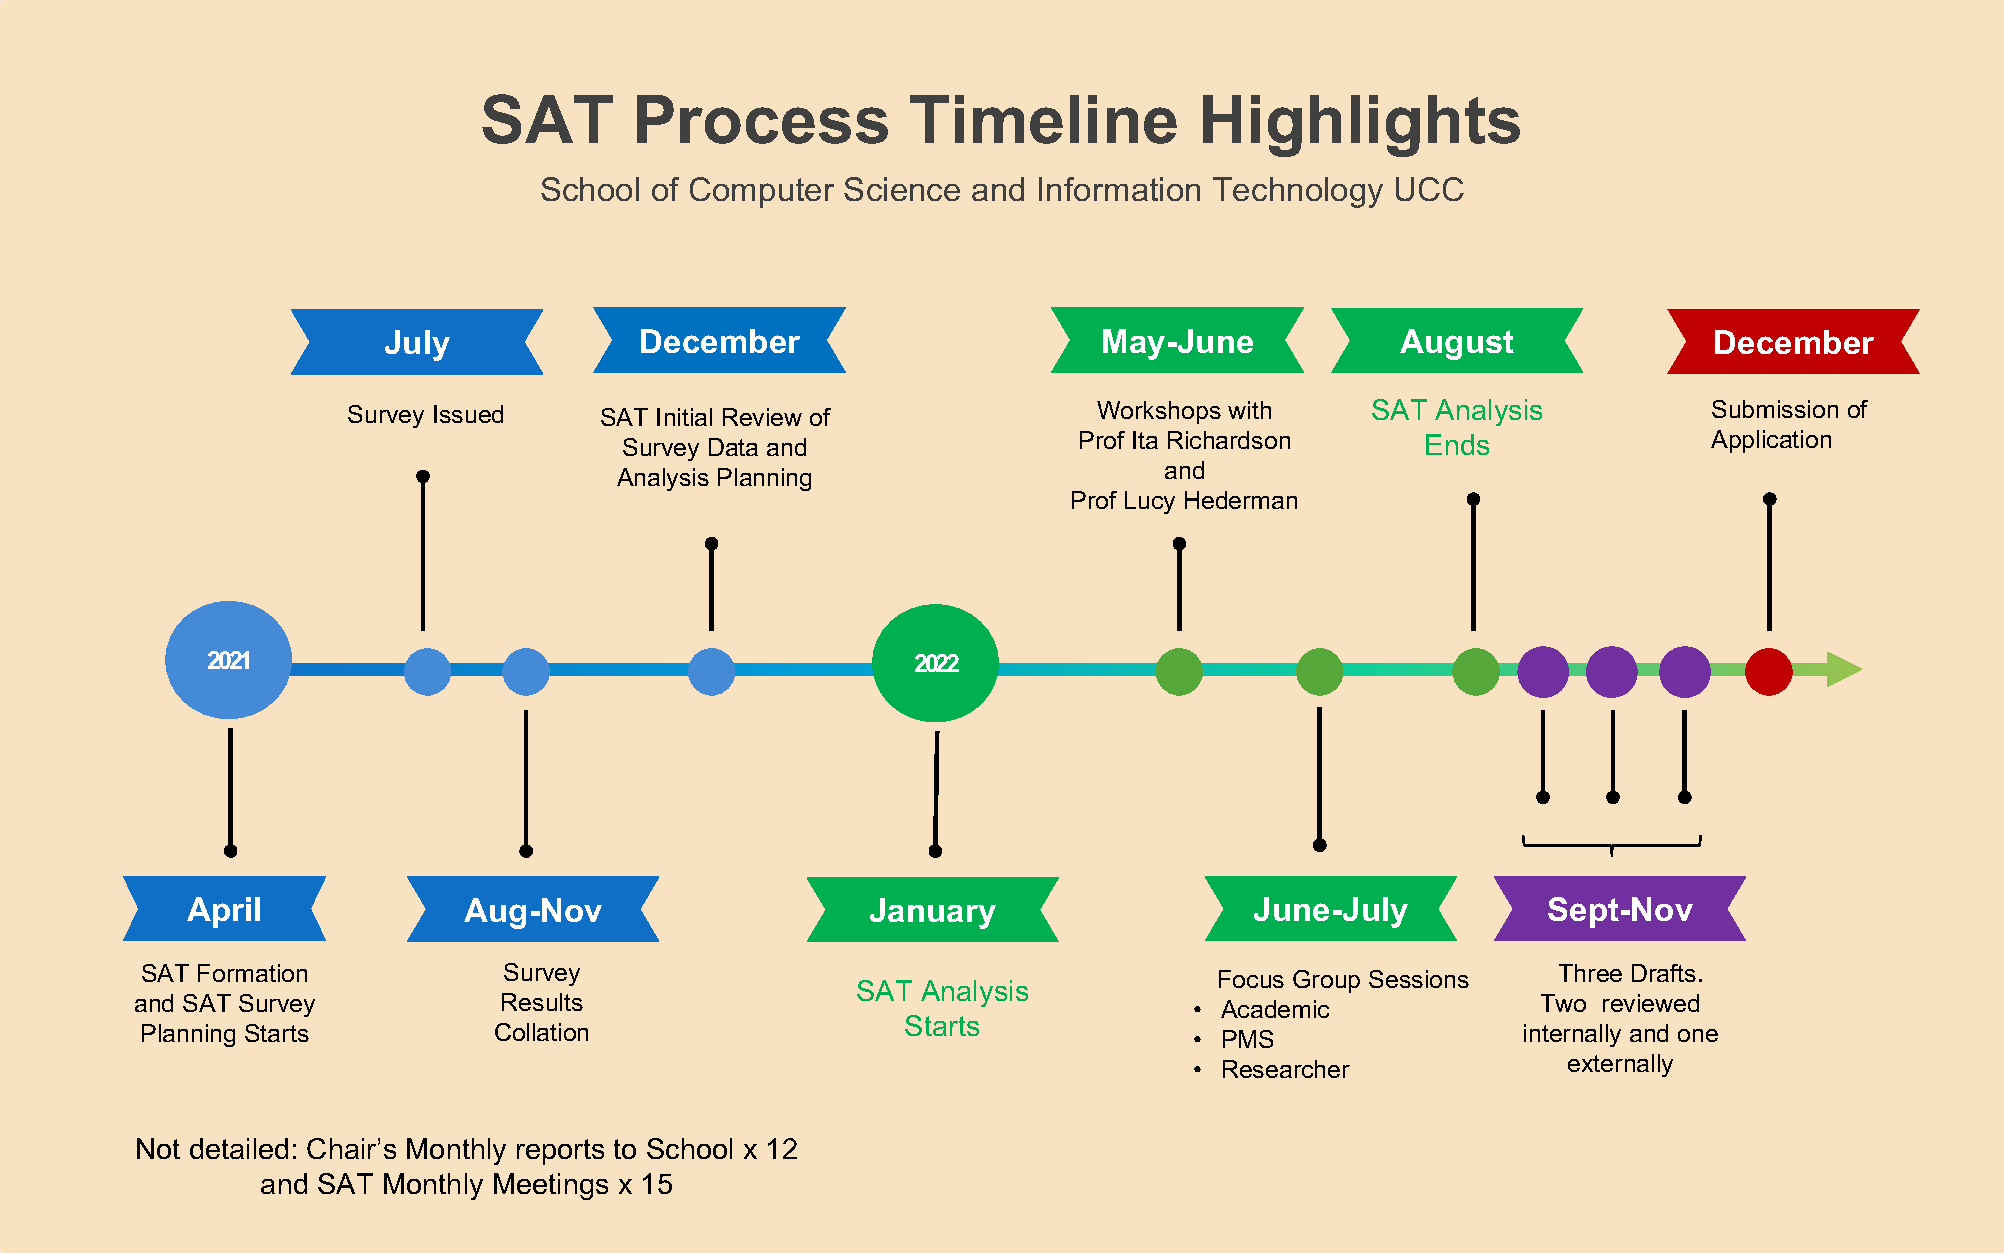
\includegraphics[trim={3mm 3mm 3mm 3mm},clip,width=20cm]{fig/timeline2.pdf}
    
\end{figbox}

\end{landscape}





\subsubsection{Information on how the findings and activity of the self-assessment team are, and will continue to be, communicated to senior management and the wider department}

The EDIIC will be responsible for evaluating progress and for overseeing the implementation of the action plan.
The EDIIC will meet monthly, to review progress, measure success and impact and take any actions necessary to progress the action agenda. The EDIIC Chair will report bi-annually to the school (Action~\ref{action:intro:agenda}).
The EDIIC will act as the main conduit between the school and  the College's EDI committee.



\begin{actionblock}{\ksspace{}Continuous updates to school}{intro:agenda}
\actintroagenda
\hfill{
    \hypersetup{hidelinks}
    \hyperlink{a5}{\gotoactionsymbol{}}
}
\end{actionblock}




In addition, to gauge the cultural impact of the AS implementation plan on staff and students, the EDIIC will conduct a review in 2026
(Action~\ref{action:intro:review:year3}).

\begin{actionblock}{\ksspace{}Review AS impact Year 3}{intro:review:year3}
\actreviewimpactyearthree
\hfill{
    \hypersetup{hidelinks}
    \hyperlink{a6}{\gotoactionsymbol{}}
}
\end{actionblock}





